\documentclass[12pt]{article}
\usepackage[a4paper,total={6in,9in}]{geometry}
\usepackage{wrapfig}
\usepackage{graphicx}
\usepackage{amssymb}
\usepackage{mathtools}
\usepackage{listings}
\usepackage{url}
\usepackage{hyperref}
\usepackage{xcolor}

\author{\textbf{Anshuman Singh} \\ \textbf{2018JTM2004}\\ \textbf{2018-19}}
\date{}
\title{\textbf{Assignment-8\\ELP- 718 Telecom Software Laboratory}}

\begin{document}
	\maketitle
	
	\begin{center}
	\noindent \textbf{A report presented for the assignment on\\Python and GitHub }
	\vspace{1cm}
	
	\begin{figure}[h]
	\centering
	
\includegraphics[scale=.2]{iitd.jpg}
	
	
	\end{figure}
	\vspace{1.5cm}
	
	\textbf{Bharti School\\of\\Telecommunication Technology and Management\\IIT DELHI, Delhi\\September 27, 2018}
	
	\end{center}
	
	\newpage
	\tableofcontents
	\listoffigures
	\newpage
	
	\section{Problem Statement-1}
	
	
		\subsection{Problem Statement}
		IIT Delhi, has just got the strongest computer. The professors in charge wants to check the
		computational capacity of the computer. So, they decided to create the problem which is to
		be given as an assignment to students. Can you help the professor to check the computation
		capability of the computer?
		
		A valid cross is defined here as the two regions (horizontal and vertical) of equal lengths
		crossing over each other. These lengths must be odd, and the middle cell of its horizontal
		region must cross the middle cell of its vertical region.
		
		
		\begin{figure}[h!]
			\centering
			\caption{Valid and Invalid crosses}
			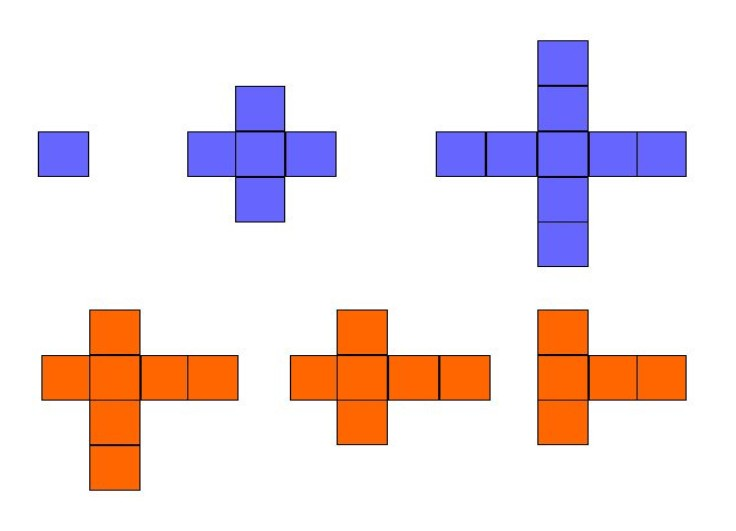
\includegraphics[scale=.5]{ps1_p_1.jpg}
		\end{figure}
		
		In the diagram above, the blue crosses are valid and the orange ones are not valid.
		Find the two largest valid crosses that can be drawn on smart cells in the grid, and return
		two integers denoting the dimension of the each of the two largest valid crosses. In the
		above diagrams, our largest crosses have dimension of 1, 5 and 9 respectively.
		\textbf{Note:} The two crosses cannot overlap, and the dimensions of each of the valid crosses
		should be maximal.	
		\subsection{Constraints}
		
			\begin{itemize}
				\item $2<=n<=105$
				\item $2<=m<=105$
			\end{itemize}
		
		\subsection{Algorithm and Implementation~\cite{problem2}~\cite{problem1}}
		
			\begin{itemize}
				\item Create a file ps1.py
				\item First ask for no. of columns and rows in the given input pattern of S and D
			    \item Then read the entered rows and columns in a two dimensional list.
			    \item Using various for loops determine the number of crosses present and their size.
			    \item Print the cross with maximum and minimum size.
			\end{itemize}

		\subsection{Flow Chart}
		
			\begin{figure}[h!]
				\centering
				\caption{Flow Chart for Figure 1}
				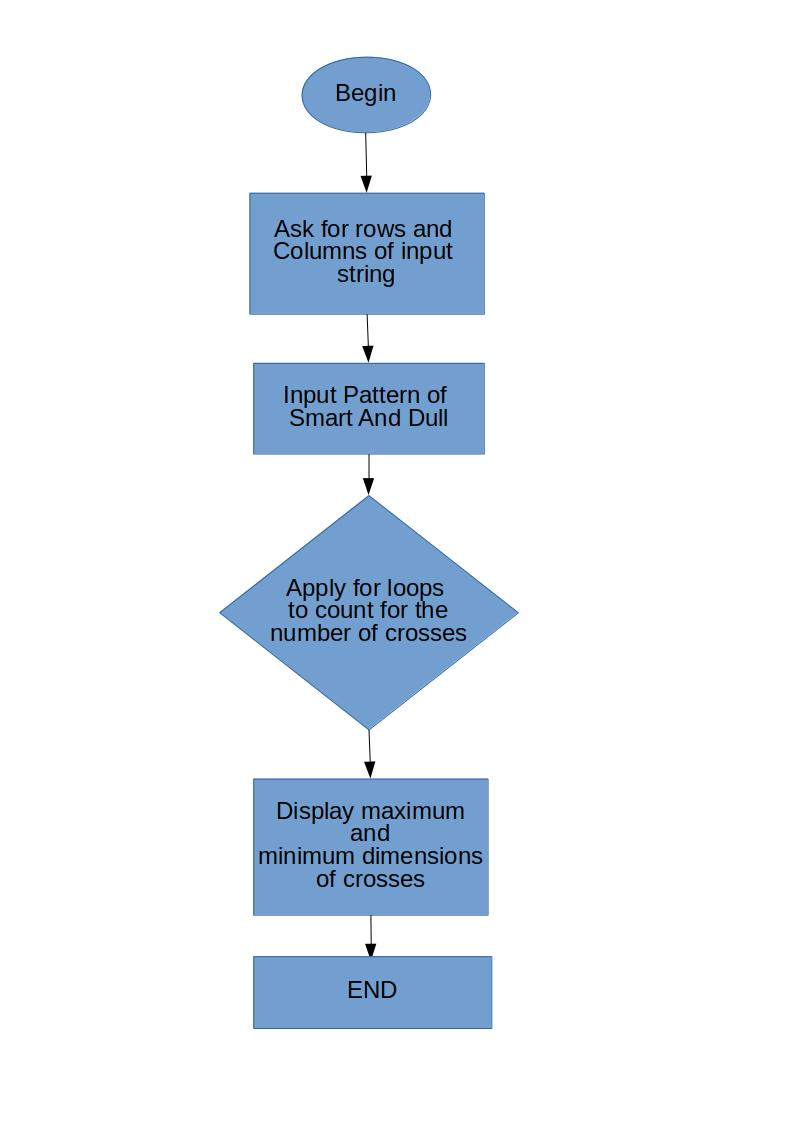
\includegraphics[scale=.5]{ps1_f_1.jpg}
			\end{figure}

		\subsection{Input and Output Format}
		
			\begin{itemize}
				\item Input Format:\\The first line contains two space-separated integers, n and m.
				Each of the next lines n contains a string of m characters where each character is either S
				(Smart) or D (Dull). These strings represent the rows of the grid. If the jth character in the ith
				line is S, then (i,j) is a cell smart. Otherwise it's a dull cell.
				\item Output Format:\\ Find two valid crosses that can be drawn on smart cell of the grid, and return the dimension
				of both the crosses in the reverse sorted order(i.e. First Dimension should be the larger one
				and other should be smaller one)
				\begin{enumerate}
					\item Sample Input 1
					\subitem 5 6
					\subitem SSSSSS
					\subitem SDDDSD
					\subitem SSSSSS
					\subitem SSDDSD
					\subitem SSSSSS
					\item Sample Input 2
					\subitem 6 6
					\subitem DSDDS​D
					\subitem SSSSSS
					\subitem DSDDSD
					\subitem SSSSSS
					\subitem DSDDSD
					\subitem DSDDSD
				\end{enumerate}

			\end{itemize}

		\subsection{Screenshots}
		
			\begin{figure}[h!]
				\centering
				\caption{Terminal Output of Problem 1}
				%\includegraphics[scale=.5]{ps1_1.jpg}
			\end{figure}

	\section{Problem Statement-2}
	
		\subsection{Problem Statement}
		After, getting mix results of valid crosses, professors decided to test the computation abilities
		on one more problem. This time professors wanted to test the decryption capabilities of the
		computer.
		
		Encryption of a message requires three keys, k1, k2, and k3. The ​26 letters of English and
		underscore ​ are divided in three groups, ​[a-i] form one group, [j-r] a second group, and
		everything else ([s-z] and underscore) the third group ​. Within each group the letters are
		rotated left by ki positions in the message. Each group is rotated independently of the other
		two. Decrypting the message means doing a right rotation by ki positions within each group.
			\begin{figure}[h!]
				\centering
				%\includegraphics[scale=.6]{}
			\end{figure}
			
		\subsection{Constraints}
		
			\begin{itemize}
				\item $1 <= Length of the string <=150$
				\item $1<= ki <=150 (i=1,2,3)$
			\end{itemize}
		
		\subsection{Algorithm and Implementation~\cite{problem2}~\cite{problem3}}
		
			\begin{itemize}
			\item Create a file ps2.py
			\item Ask for the encryption keys K1, K2, K3.
			\item Separate the input string into three parts as per the defined grouping.
			\item Rotate the groups by the specified keys.
			\item Then print the decrypted message by combining different groups after rotating it corresponding to the original bit position.  
			\end{itemize}
		\newpage
		\subsection{Flow Chart}
			\begin{figure}[h!]
				\centering
				\caption{Flow Chart of Problem 2}
				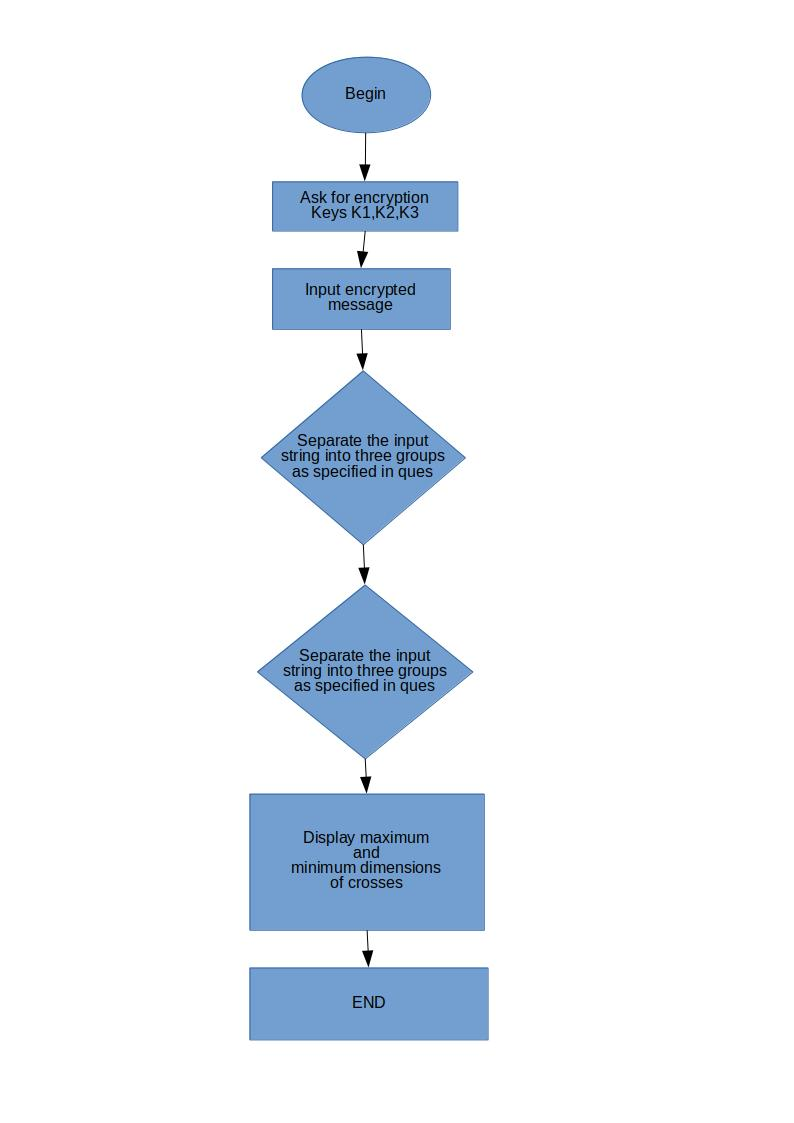
\includegraphics[scale=.6]{ps2_f_1.jpg}
			\end{figure}
		
		\subsection{Input and Output Format}
			\begin{itemize}
				\item \textbf{Input Format:} All input strings comprises of only lowercase English alphabets and underscores(\_) 
				\item  \textbf{Output Format:} For each encrypted message, the output is a single line containing the decrypted string.
				\begin{enumerate}
					\item \textbf{Sample Input 1}
					\subitem 2 3 4
					\subitem dikhtkor\_ey\_tec\_ocsusrsw\_ehas\_
					\item \textbf{Sample Output 1}
					\subitem hardwork\_is\_the\_key\_to\_success
					
				\end{enumerate}
			\end{itemize}
		
	
			
			
			
				
				
		\subsection{Screenshots}
		
			\begin{figure}[h!]
				\centering
				\caption{Terminal Output of Problem 2}
				%\includegraphics[scale=.5]{ps2_1.jpg}
			\end{figure}
		
	\section{Appendix}
	
	
		\subsection{Code for ps1}
		
			\begin{verbatim}
			\end{verbatim}
			\lstinputlisting[]{ps1.py}
		
		\subsection{Code for ps2}
		
			\lstinputlisting[]{ps2.py}
		
		\bibliographystyle{plain}
		\bibliography{report.bib}

\end{document}
